\documentclass[noraggedright]{turabian-researchpaper}

% Turabian Formatting
\usepackage{turabian-formatting}

% Chicago Bibliography Formatting
\usepackage[
  autocite = footnote,
  sorting=ynt,
  annotation]
  {biblatex-chicago}
   
\renewcommand{\bibfont}{\normalsize}
\addbibresource{Bibliography.bib}

% Language and Text Formatting
\usepackage[utf8]{inputenc}
\usepackage[T1]{fontenc}
\usepackage{microtype}
\usepackage[greek, english]{babel}
  \babeltags{en = english}
  \babeltags{el = greek}
\usepackage{teubner}

% Packages recommended for Turabian
\usepackage{threeparttable}
\usepackage{ellipsis}
\usepackage{tocloft}
\usepackage{csquotes}

% Title Page
\title{This Great Flood of Words\thanks{Rep. 1: 344 d1}}
\subtitle{A Brief Phasal Analysis of the Dialogue
  between Socrates and Thrasymachus}
\author{Thomas Broadwater}
\course{GREK 8010: Readings and Research in Greek Literature}
\submissioninfo{}
\date{\today}

\usepackage{Sweave}
\begin{document}
\Sconcordance{concordance:GreatFlood.tex:GreatFlood.Rnw:%
1 39 1 1 0 2 1 1 11 1 19 1 12 1 5 140 1 1 180 10 1 1 2 12 0 1 2 6 1 2 2 %
6 1 1 2 12 0 1 2 4 1 2 2 31 1 1 92 5 1 1 2 12 0 1 2 6 1 2 2 17 1 1 11 1 %
2 43 1}






\maketitle

\input{Sections/Methodology.Rnw}
%\input{Sections/Sentences.Rnw}

\section{Sentences per Turn (Turn Density)}



The first portion of the code tallies the number of sentences per turn, hoping
to identify a correlation between turn ``density'' and the occurrence of phase
transitions. It counts the data in two ways. First, it gathers ``global''
calculations, i.e., the relevant information from the entire dialogue, and
second, it gathers speaker-by-speaker calculations. In order to construct a
high-level view of turn density, the script returns a table of calculations.
The mean represents the average number of sentences per turn, the median
represents the middle value when the data is organized numerically, and the mode
represents the middle value when organized. The standard deviation represents
the overall variation within the data. The table is printed below.

\begin{table}
\begin{Schunk}
\begin{Soutput}
# A tibble: 6 × 5
  speaker      mean median  mode    sd
  <chr>       <dbl>  <dbl> <int> <dbl>
1 global       1.69    1       1 1.79 
2 cleitophon   1.33    1       1 0.577
3 glaucon      1.25    1       1 0.463
4 polemarchus  1.75    1.5     1 0.957
5 socrates     1.99    1       1 1.90 
6 thrasymacus  1.41    1       1 1.72 
\end{Soutput}
\end{Schunk}
\caption{Turn Density Data}
\label{tab:DensityData}
\end{table}

The table shows notably regular results. Each speaker's average sentence
density is close to the global, $\bar{x}_g = 1.68$. Cleitophon and Socrates
deviate the most, $\bar{x}_c = 1.33$ and $\bar{x}_s = 1.99$, respectively, but
the variations are slight, making it difficult to tell what difference is
significant. The script performs a t-test comparing the global mean to each
speaker's to solve this problem. This test will return a figure called a
p-value for each speaker. For the purposes of this study, if a p-value is less
than 0.05, then the difference between the speaker's mean and the global mean
are significantly different. The results of the test are printed below.

\begin{table}
\begin{Schunk}
\begin{Soutput}
[1] "cleitophon: 0.0755533142252797"
[1] "glaucon: 0.0953570075963998"
[1] "polemarchus: 0.0102844982210078"
[1] "socrates: 0.0514802153411887"
[1] "thrasymacus: 0.0581347985214711"
\end{Soutput}
\end{Schunk}
\caption{P-Values: Average Turn Density by Speaker}
\label{tab:DensityPval}
\end{table}

Interestingly, Only Polemarchus shows a statistically significant deviation from
the global mean. In Polemarchus' case, the small sample size may skew the data.
Polemarchus only has four turns in the entire dialogue. His third turn (P3) is
three sentences long, P2 is two sentences long, and P1 and P4 are both one
sentence long. As such, his result here provides little insight. 

Without any useful p-values to rely on, it becomes helpful to visualize the
data. Below is a histogram representing each turn in the order of occurrence.
The x-axis represents the index — a number identifying each turn in the data
set — and the y-axis represents the number of sentences in each turn. The blue
line represents the global mean density over time.

\begin{figure}
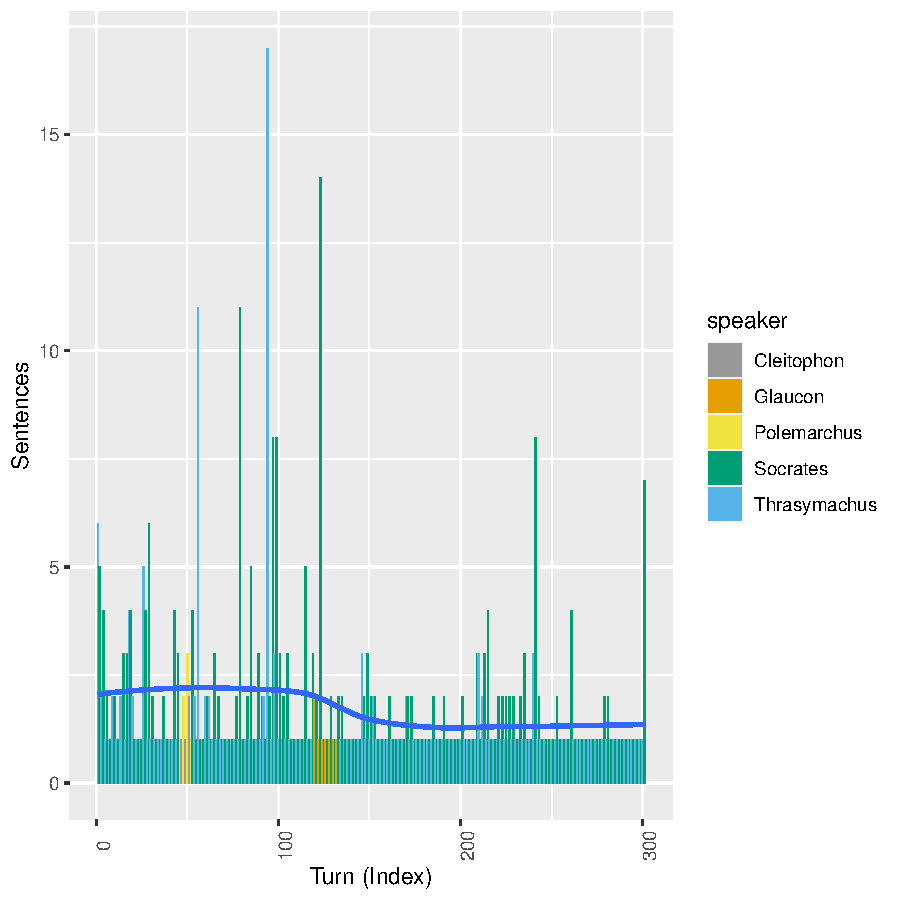
\includegraphics{GreatFlood-Turn_Conseq}
\caption{Sentence Density by Speaker}
\label{graph:SentenceDensity}
\end{figure}

As reported by the initial data, the dialogue shows a consistent regularity in
sentence density. However, Socrates and Thrasymachus both show greater variation
than the others, especially in the early half of the text. 
This variation is measured by the standard deviations above. A similar t-test on
them reveals that both have a significantly high range of sentence densities:
$\sigma_s = 0.02$ and $\sigma_t = 0.01$ (both rounded), respectively. These
p-values imply that significantly denser turns than the average should be
considered when defining phases.

\begin{table}
\begin{Schunk}
\begin{Soutput}
[1] "cleitophon: 0.301818447656808"
[1] "glaucon: 0.339266024338994"
[1] "polemarchus: 0.187958111608137"
[1] "socrates: 0.0175810404193463"
[1] "thrasymacus: 0.0129304749109537"
\end{Soutput}
\end{Schunk}
\caption{P-Values: Standard Deviation of Turn Density by Speaker}
\label{tab:SDPval}
\end{table}

\end{document}
